\documentclass{article}
\usepackage[utf8]{inputenc}
\usepackage[pdftex]{graphicx}
\usepackage{amsmath}
\usepackage{amsfonts}
\usepackage{amssymb}
\usepackage{pdfpages}
\usepackage[font=small]{caption}
\usepackage{float}
\usepackage{comment}
\usepackage{setspace}
\usepackage{gensymb}
\usepackage{multicol}
\usepackage{fancyhdr}
\usepackage{enumitem}
\usepackage{mathtools}
\usepackage{natbib}
\usepackage[titletoc,title]{appendix}

\paperheight 11in
\paperwidth 8.5in
\marginparwidth 0in
\hoffset 0in
\oddsidemargin 0in 
\evensidemargin 0.25in 
\marginparsep 0.25in
\topmargin 0.25in 
\textwidth 6.5in \textheight 8.5in
\renewcommand{\baselinestretch}{1.15}
\setlength{\parindent}{0em}

\title{Modeling Refugee Immigration Policies \\ \\ \large MCM: Problem F}
\author{Graham Pash, Ken Jutz, Jay Sudweeks}
\date{February 1, 2016}   

\pagestyle{myheadings}
\pagestyle{fancy}
\fancyhf{}
\renewcommand{\headrulewidth}{0pt}
\rhead{Page \thepage \\ Team 50318}

\begin{document}

\maketitle

\begin{abstract}

\noindent Recent conflict in Syria  has driven millions of citizens from their homes,  resulting in a record number of refugees throughout Europe\cite{CNN2}. Relocating and settling all refugees will take effective policy and resource allocation. We constructed a network equilibrium model of the flow of refugees and resources throughout Europe, North Africa, and the Middle East. Specifically, the movement of refugees from their places of origin through 6 main routes to Europe were considered, as well as their eventual resettlement in European host countries. This model was constructed keeping in mind the possibility of a crisis such as this occurring anywhere in the world due to social or political unrest, natural disaster, or another unforeseen event. Thus the model has been generalized to allow for the  effortless addition of additional locations. Furthermore, our model includes a realistic simulation of refugee decision making, which includes a variety of factors including distance, stability of a potential host country, as well as measures of the standard of living in these countries. This algorithm provides an accurate model of refugee movement. A similar network model for aid is coupled with this model to determine ideal distribution of international funds to stabilize the situation in the shortest amount of time possible. From the results of this model, a report has been prepared containing policy recommendations to the UN Secretary General and the Chief of Migration on how to stabilize future situations much more quickly.

\begin{enumerate}
    \item Prioritize large standing refugee populations over large transient populations
    \item Supplement domestic aid money with international aid funds to resettle refugees
    \item Distribute resources over time instead of a lump sum delivery
    \item Anticipate arrival regardless of travel condition and refrain from wasting funds on infrastructure
    \item Prioritize transient countries only if the flow of refugees would destabilize the country, otherwise allocate funds for infrastructure during calm periods


    
\end{abstract}

\pagebreak

\noindent Dear UN Secretary General and the Chief of Migration,\\

The refugee crisis occurring in Europe is a matter that concerns us all. The safe and efficient relocation of displaced persons not only improves the quality of life of refugees, but also lowers the likelihood of further conflict between origin and host nations. 
Managing this crisis will take effective policy and resource allocation. To this effort, we have created a model of the flow of refugees and resources throughout Europe, North Africa, and the Middle East to help inform your policy making decisions. Our model focuses on relocating refugees to a place that provides them with a long term place to stay, and also with an acceptable quality of life.\\
Based on the results of the model, we suggest the following policy actions:
\begin{enumerate}
    \item Prioritize standing refugee populations over large transient populations. In other words, the countries that hold a large standing population should be given more aid than those countries that serve as a way point, even if way point countries do experience more refugees. Refugees pass through way point countries relatively quickly. Thus, aid in these locations will not help them for very long. However, if aid is concentrated in areas where populations rest for a longer, refugees will benefit from this aid for longer. 
    \item Supplement domestic aid money with international aid money. In other words, instead of using aid to help refugees move, allocate the money to help refugees settle once they have reached their final locations. This allows for permanent resettlement, which creates stability.
    \item Distribute resources over time, instead of allocating them all at once. This allows aid distribution to develop with the dynamics of the crisis. It is very difficult to predict where a crisis will occur. If resources are allocated all at once, then there is very little flexibility for responding to unforeseen events. However, if resources are allocated over time, there is a potential for elasticity in resources to be distributed where they are needed most.
    \item Anticipate arrival regardless of travel condition. Infrastructure can be improved with excess funds, but aid should not be used initially for this purpose. 
\end{enumerate}
\\
There is of course one stipulation with the last suggestion. While expanding travel routes during the middle of a crisis is extremely inefficient, if the amount of refugees flocking to these countries reaches a threshold that would destabilize the whole region, it may become a necessity. Even in the case of a large scale crisis such as the current situation regarding Syrian refugees, it would be inefficient to allocate funds on infrastructure or transportation of refugees as they will continue to find a way to flee from their country. Rather this money should be focused on settling refugees once they have reached their final destinations. However, if the scale of the crisis were say ten times that of the current crisis, it would be of paramount concern that refugees move swiftly to avoid standing refugee populations in neighboring countries that would destabilize the entire region. We have determined that it is only in extreme cases such as this that we suggest considering the immense cost to build new transportation networks or to relocate refugees to countries such as China and the United States via aircraft and other expensive modes of travel.\\
\noindent We sincerely hope that our report is of use,\\

\noindent ICM Refugee Analytics, Team 50318

\pagebreak

\setlength\parindent{0pt}

\section{Introduction}
A refugee is one who leaves his home country to escape persecution or danger\cite{10.2307/3002424}. There are many factors which force people to flee their countries, including natural disasters and political and social unrest. Recently, refugees have flooded Europe, as the war in Syria has pushed refugee numbers to record highs\cite{CNN2}. Many of these refugees are vulnerable, with more than half of the refugee population comprised of children\cite{CNN2}. As refugees pour into Europe, in numbers estimated to be as high as 8,000 a day\cite{BBC8000}, it becomes increasingly clear that Europe does not currently have the policy or structure in place to handle this increasing demand, and so refugees risk their lives every day in search of a better life, only to be turned away or left stranded in bureaucratic purgatory\cite{BBC8000}. This is a pressing issue that demands immediate action and solution, not only so that refugees can begin to rebuild their lives, but also so that tensions between refugees home countries and asylum countries are eased.

\section{Analysis of the Problem}
To solve this daunting problem, one must first analyze the movements of refugees, and then secondly distribute aid resources to enable a better quality of life for refugees.\\
When modeling the movement of refugees, it is important to keep in mind that these are people whose lives are by nature chaotic. While in theory we would like to model a refugee as someone who makes a perfectly rational decision at each step along their path, this is simply not the reality. Refugees often have little time to thoroughly evaluate their choices. Thus, to appropriately model movement, and to advise policy that will be effective in real world scenarios, one must attempt to understand the thought process and factors that determine where a refugee will travel. This can only be modeled by determining a list of select metrics, which should emulate those that a refugee would consider.\\
To determine where to focus aid resources to have the maximum impact, it is important to realize the role that aid plays in a dynamic model. Since there is no accurate way to predict where crises may occur, aid plays a "chasing" role-- aid moves to help the people where it can; in turn refugees will move towards countries where aid is being given. Thus to effectively model this, there must be some form of feedback loop between resources and people.\\
With this in mind, our model should focus on moving people towards countries with more resources and higher standards of living; however, it should also balance numbers so that a given country is not overloaded with refugees.\\
Once this model has been established, it would be able to inform policy to support the movement of refugees and stabilize the situation. This policy would be informed by the movement of refugees through countries, as well as the aid that can be expected if a crisis were to occur. \\
It is important to understand that this is not merely a thought experiment. Rather, it is a tool to ease the suffering of many millions of people worldwide. The model should not overlook the critically important human element intrinsically tied to any theoretical solution of this problem.


\section{Assumptions and Justifications}
\begin{itemize}

\item \textbf{Assumption 1:} A refugee's decision and subsequent movement is a discrete process.
\noindent \textbf{Justification:} For our model, it was not computationally feasible to model the decision making processes and movement of refugees as continuous. This is acceptable, however, as the we have chosen a time step large enough to allow for the movement of waves of people, but small enough so that the information that each refugee receives is current.

\item \textbf{Assumption 2:} Some countries need not be added to the network.\\
\noindent \textbf{Justification:} Since countries such as Eritrea are not a primary destination of refugees from say, Syria, we have left the directional connection from Syria to Eritrea off of our network. Similarly, we are not modeling movement through intervening countries between hubs and source nodes. For example, a refugee that intends to move from Syria to Libya so that they may take the Central Mediterranean path to Europe would simply be moving through Egypt, not intending Egypt as a final destination. Thus the Syria to Egypt connection has been left off of our network, to keep refugees in our model from residing in countries that are not reasonable locations.

\item \textbf{Assumption 3:} No births or deaths occur during the journey.\\
\noindent \textbf{Justification:} Since it is not easily researched how many births or deaths occur for refugees en route to their final destination, we have omitted including this to avoid forcing upon our model an unrealistic constraint. 

\item \textbf{Assumption 4:} Resources are liquefied into a monetary amount. Additionally, distributed aid is used to purchase individual resources, such as food, water, and medicine in perfect amounts.\\
\noindent \textbf{Justification:} Due to difficulty of researching and determining the amount of resources such as food, water, medicine and intangibles such as education, emotional support, etc. needed by a single refugee, we were forced to account for resources in a reliable way, namely through money. A monetary value needed by a refugee can easily be found. However, it must be assumed that this dollar amount encompasses all of the individual resources needed, and nothing is left out, i.e. it is not the case that too much money is spent on food and thus medicine cannot be purchased.

\item \textbf{Assumption 6:} The time of the year does not matter.\\
\noindent \textbf{Justification:} Since refugees primary concern is to move from their ravaged home country, we have assumed that weather is not a deterrent to their movement.

\item \textbf{Assumption 7:} The scaling of our cost and utility functions does not matter, as long as they are on the same scale.\\
\noindent \textbf{Justification:} Although one may be concerned of a possible clustering of countries if the scale used for cost or utility is not great enough, Linear Algebra assures us that scalar coefficients do not change the solution of a system of equations.

\item \textbf{Assumption 8:} Every country spends a fixed percentage of its GDP on refugees residing in their country each year.\\
\noindent \textbf{Justification: } Since it is not feasible to read the budget of every country in the network to find the monies allocated to aid refugees in their own country, we had to assume there was a standard percentage of GDP that every country allotted for. Furthermore, the yearly amount for this aid is distributed evenly throughout the year.

\item \textbf{Assumption 9:} All international aid comes from a common source.\\
\noindent \textbf{Justification: } Since the solution to this crisis depends on the collaboration of many countries, it would make sense for a board to be created to handle the organized distribution of relief funds, namely the United Nations. A result of this is that aid does not flow between borders.

\item \textbf{Assumption 10: } Resource distribution is an immediate process.\\
\noindent \textbf{Justification: } Since resources have been liquefied to a dollar amount, this money can be transferred immediately, so that by the end of the one week time step used in our model, it will have already been distributed. Thus the funds will be in place for the next time step.

\item \textbf{Assumption 11: } Each country can only take a certain proportion of its indigenous population in as refugees, and this is the capacity for refugees.\\
\noindent \textbf{Justification: } This makes sense, because if a country allows too many refugees in its country, it risks sparking social unrest within its own borders. For simplicity, this was set as a set percentage of the population.

\end{itemize}

\section{Modeling Relocation of Refugees}
\subsection{Metrics of Refugee Crises}
Our model focuses on a sustainable relocation of refugees. Thus, we must consider both the ability of a given refugee to move and the capacity of a country to take in and support that refugee over time. \\

\textbf{Factors that Influence Refugee Movement}
\begin{enumerate}
    \item \textbf{Distance:} A refugee must consider the distance between where she is and where she is interested in going.
    \item \textbf{Resource Need:} A refugee cannot move if she has not met her basic needs, or if the place that she wants to move to cannot meet those needs. It is important to note that it is advantageous to be in another location with more resources available to remain in one where there are fewer resources.
    \item \textbf{Safety of Route:} Before a refugee moves, she must assess the safety of her possible routes. Ideally, a refugee would move along the safest path. 
    \item \textbf{The Human Development Index: } The Human Development Index (HDI) is a measure of a country’s achievement in terms of its people and their capabilities \cite{HDI}. HDI is a measure of the quality of life inside of a given country. A refugee should want to move towards countries with favorable HDI scores. 
\end{enumerate}
\\
\textbf{Factors that Influence a Country's Capacity}
\begin{enumerate}
    \item \textbf{The Fragile States Index:} The Fragile States Index (FSI) is a measure of a country's stability \cite{FSIArt}. The internal stability of a country influences its ability to accept refugees.  .
    \item \textbf{Domestic Aid:} The amount of money that a given country apportions to support refugees influences the quantity of refugees that the country can accept.
    \item \textbf{International Aid:} The availability of international aid to a given country influences how many refugees that country can support.
    \item \textbf{Refugee Cap:} Realistically, a country can only absorb so many refugees before its stability is compromised. Thus, each country should have a cap value of refugees that it can welcome. 
\end{enumerate}

\subsection{Overview of the Model}
Our model is inspired by a network equilibrium framework for human migration developed by J. Pan and A. Nagurney \cite{model1}. The initial parameters at each of our location nodes and travel routes are drawn from 2014 data. A directional network is created by allowing refugees to move from their starting nodes, i.e. countries that are producing refugees, to hubs that then allow them to move to Europe. These connections are made based upon what would geographically be feasible for these refugees. Thus we have omitted the connection from Syria to Hungary, since it would not make since for a refugee to move into Asia, only to turn towards Europe when there are more direct, established routes of travel, such as stopping in Turkey along the way. The model moves in discrete steps and at each step determines population flow and resource allocation between locations based on the utility of the locations and cost of each path. We adjusted the parameters in our model so that each step resembles 1 week of time. A picture of the network is below. Also note that the six paths that we were specifically tasked to evaluate are bolded and in different colors.

\begin{figure}[H]
    \centering
    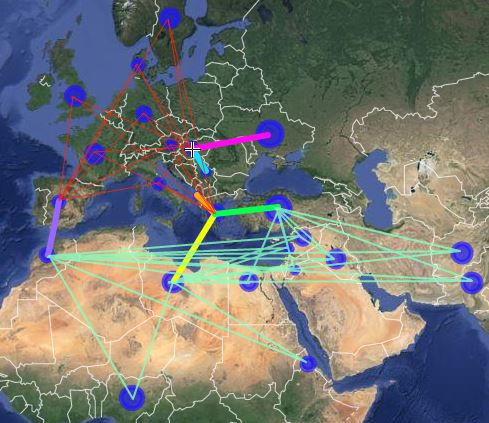
\includegraphics[width=0.6\textwidth]{NetworkPics/fully-connected.JPG}
    \caption [width=0.8\textwidth]{\centering Network used to model refugee population movements\\ (Note: directional connections have been omitted)}
\end{figure}

The locations on our map were given numbers to aid computation, and the table of these can be found as Figure 1 in the Appendix. The adjacency matrix for this network is given by Figure 2 in the Appendix.

\subsection{Establishing Cost and Utility of Refugee Movement}
Incorporating the cost and utility framework developed by the aforementioned Pan and Nagurney, we utilized the idea of a cost for movement along a selected edge and the utility, i.e. the advantage of doing so, to simulate the decision making process of refugees. The network equilibrium equation is given by:
\begin{equation}
    u_i(p)+c_{ij}(f) \begin{cases} =u_j(p) & \mbox{if } f_{ij}>0\\ \geq u_j(p) & \mbox{if } f_{ij}=0 \end{cases}
\end{equation}
where $f_{ij}$ denotes the flow from location $i$ to location $j$. Furthermore, $u_i$ is the utility function associated with location $i$ and $c_{ij}$ is the cost function associated with traveling from location $i$ to location $j$. We can see that if the utility outweighs the cost, then the flow will be nonzero, i.e. people will move. The number is associated with the flow, and is the number that balances this system of equations. Since this reduces to a system of equations in the end, it is easily solved by matrix methods, once the cost and utility functions have been defined.

We define the cost and utility at time step $n$, denoted by the superscript, by the functions as given below:
\begin{equation}
    u_i^n(p) = \frac{cap_i-p_i^n}{cap_i} + \frac{HDI_i}{max\{HDI_j\}} + \frac{120-FSI_i}{max\{FSI_j\}} + \frac{r_i^{n-1}}{p_i^{n-1}}
\end{equation}

\begin{equation}
\begin{split}
    c_{ij}(f) = \frac{distance_{ij}}{max\{distance_{i*}\}} + f_{ij}(\frac{p_j^{n-1}}{cap_j})
    + \frac{safety_j}{safety_i+safety_j} \\
    +\frac{\text{logistics cost}_{ij}}{max\{\text{logistics cost}_{i*}\}} + \begin{cases} d_{ij} & \mbox{if: } (i,j) = (16,20), (15,9), (23,9) \\ 0 & \mbox{otherwise} \end{cases}
\end{split}
\end{equation}

Here $p_k^m$ denotes the population of node $k$ at time step $m$. $cap_k$ denotes the capacity for refugees at location $k$. $HDI_k$ denotes the Human Development Index at location $k$ and similarly $FSI_k$ denotes the Fragile State Index of location $k$. Furthermore, $r_k^m$ denotes the resources of location $k$ at time step $m$ (in dollar amount). $distance_{ij}$ is the distance between locations $i$ and $j$, which were standardized by collecting data from Google Maps for distances between countries. $d_{ij}$ is the death probability along the path $i$ to $j$, and is only applicable to the three paths that we have data for, namely the Central, Eastern, and Western Mediterranean \cite{BBCMigrationGraphics}. The logistics cost is the cost for a third party to send refugees to a location, and is $0$ for the Europe, North Africa, Middle East model, since these refugees are moving on their own. It is nonzero, however, when moving refugees to North America or far east Asian countries, such as China. $safety_k$ denotes the Fragile State Index rating for safety at location $k$.
Note that both cost and utility are both on the same scale of 0 to 4, except in cases of truly international travel, where the cost function biases regional travel, as it is more costly to move to distant continents, as expected.

All numbers can be found in Figure 1 of the appendix.

\subsection{Flow of Refugees}

With the cost and utility functions described above, code was written in MATLAB to solve this system and to move the refugee populations. Initial refugee populations were determined from the 2014 refugee populations determined by UNHCR \cite{Rdata}. Initial resources of countries were determined by taking a fixed fraction of the country's GDP as determined by \cite{GDP} and allocating it to refugee aid, for simplicity this was initially assumed to be 1 percent.

\subsection{Including Resources from Aid}
Intrinsically tied to the movement of refugees, however, is movement of foreign aid. To include this model, we assumed a primary holder for all of the aid to be distributed for the crisis. This number was determined from the UN Budget \cite{UNBudget} and was divided by 52 to account for the discrete step of a week used in our model. This number of USD \$36.298 million was the weekly aid allotment, and was to be distributed to countries connected to the UN. Furthermore, a US dollar amount that a refugee needs to survive for a week was determined multiplying the standard refugee stipend in the US of \$925 \cite{Resettle} by the proportion of the purchasing power index of the given country divided by that of the US \cite{CostLiving}, i.e. $\text{weekly necessity}_j=925\cdot \frac{PPI_j}{PPI_{US}}$.
Next we had to determine a method for distributing resources. Thus, we defined the Resource Need Index (RNI), where the RNI of location $i$ is given by:
\begin{equation}
    RNI_i = \frac{\frac{r_i^{n-1}}{p_i^{n-1}}}{max\{\frac{r_k^{n-1}}{p_k^{n-1}}\}}\cdot \frac{FSI_i}{max\{120-FSI_k\}}\cdot \frac{HDI_i}{max\{HDI_k\}}
\end{equation}

Next we sum up the RNI for all N countries, $\sum_{k=1}^N RNI_k$. Next we find the proportion of funds that that country should receive by $\frac{RNI_i}{\sum_{k=1}^N RNI_k}$. Thus the funds received for a given week by any given country would be:
\begin{equation}
    \text{Weekly Aid Received}_i = \$36.298 \text{ million} \cdot \frac{RNI_i}{\sum_{k=1}^N RNI_k} 
\end{equation}

Now that we have a method for distributing funds, we need to know which countries funds can be distributed to. Thus we had to create another network for aid distribution. Countries that are producing refugees were left out of this network, since these funds are designed to aid refugees, not internally displaced persons. This network can be seen below and the adjacency matrix is Figure 3 of the Appendix.

\begin{figure}[H]
    \centering
    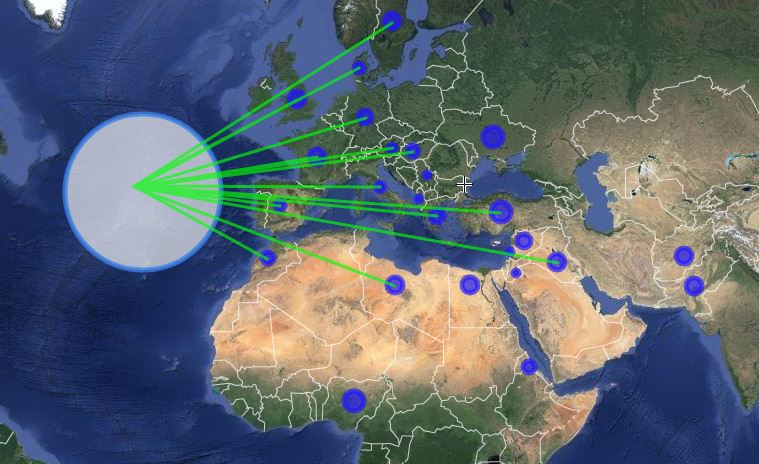
\includegraphics[width=0.6\textwidth]{NetworkPics/aid-network.JPG}
    \caption [width=0.8\textwidth]{\centering Network used to model the movement of international aid\\ (Note: directional connections have been omitted)}
\end{figure}

It is important to note that the large node over the Atlantic Ocean represents the United Nations and not an actual country. It is also important to note that the initial resources of every country replenish every step, as we divided their total by 52 weeks, so that they are distributed evenly throughout the year.

\subsection{Dynamic Model}
With all of these definitions and all of the data in place, we were able to run the MATLAB code to determine what would happen. Below is a simplified diagram of the code used to evaluate the movement of refugees and international aid monies. Note that if we wanted to model only refugee movement, we simply did not distribute resources or include the resource metrics.

\begin{figure}[H]
    \centering
    \includegraphics[width=0.8\textwidth]{modelFlowChart.png}
    \caption [width=0.8\textwidth]{Pseudo-Code for the Flow of Refugees and Resources}
\end{figure}

\section{Model Analysis}

\subsection{Movement Patterns of Refugees}

Refugee movement out of countries in crisis initially occurs very rapidly, but decreases as time goes by. We can see this occurring with Syria in the figure below. There is a huge spike of approximately 85,000 people fleeing Syria within the first week. This is expected, since as refugees flee their home country there is less unrest, and eventually the situation stabilizes.

\begin{figure}[H]
    \centering
    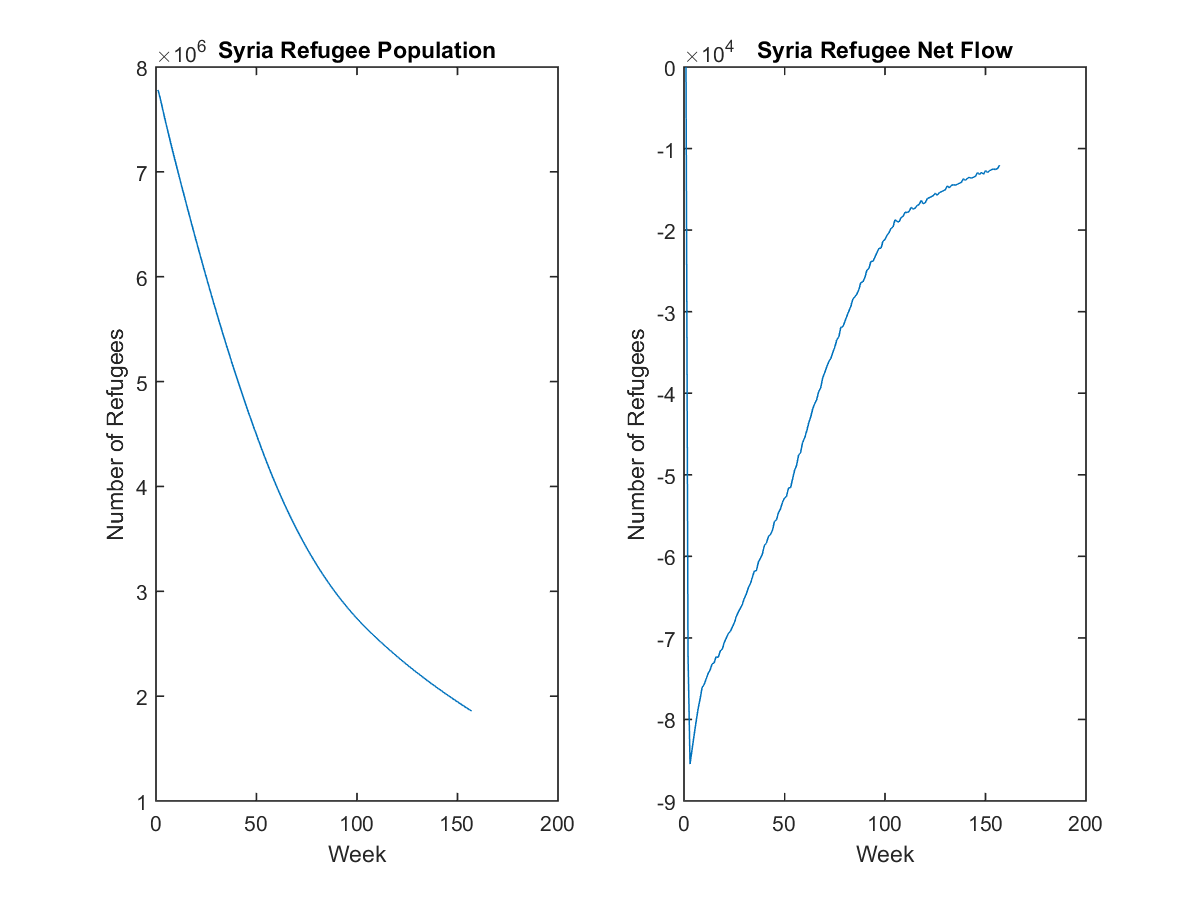
\includegraphics[width=.7\textwidth]{PostRefugeePlots/Syria_RefugeePopandFlow.png}
    \caption [width=0.9\textwidth]{\centering Syrian refugee population and flow.}
\end{figure}

Hub countries for the six main routes from North Africa, the Middle East, and Eastern Europe have some of the most interesting patterns. When the crisis first begins they receive large numbers of refugees, which eventually peaks. This occurs as the model quickly tries to move refugees through these countries to destination countries in Europe, creating a bottleneck. Partially, this is influence by the distribution of aid, which raises the capacity for refugees in these countries, which in turn increases the number of refugees that flock to these countries. Thus, there is an effect of turning these hub countries into waiting zones for further movement along the chain. As the population of refugees declines, it experiences a jagged oscillating descent, as the departure of old refugees creates room for new ones. Turkey, seen below, is a good example of this.

\begin{figure}[H]
    \centering
    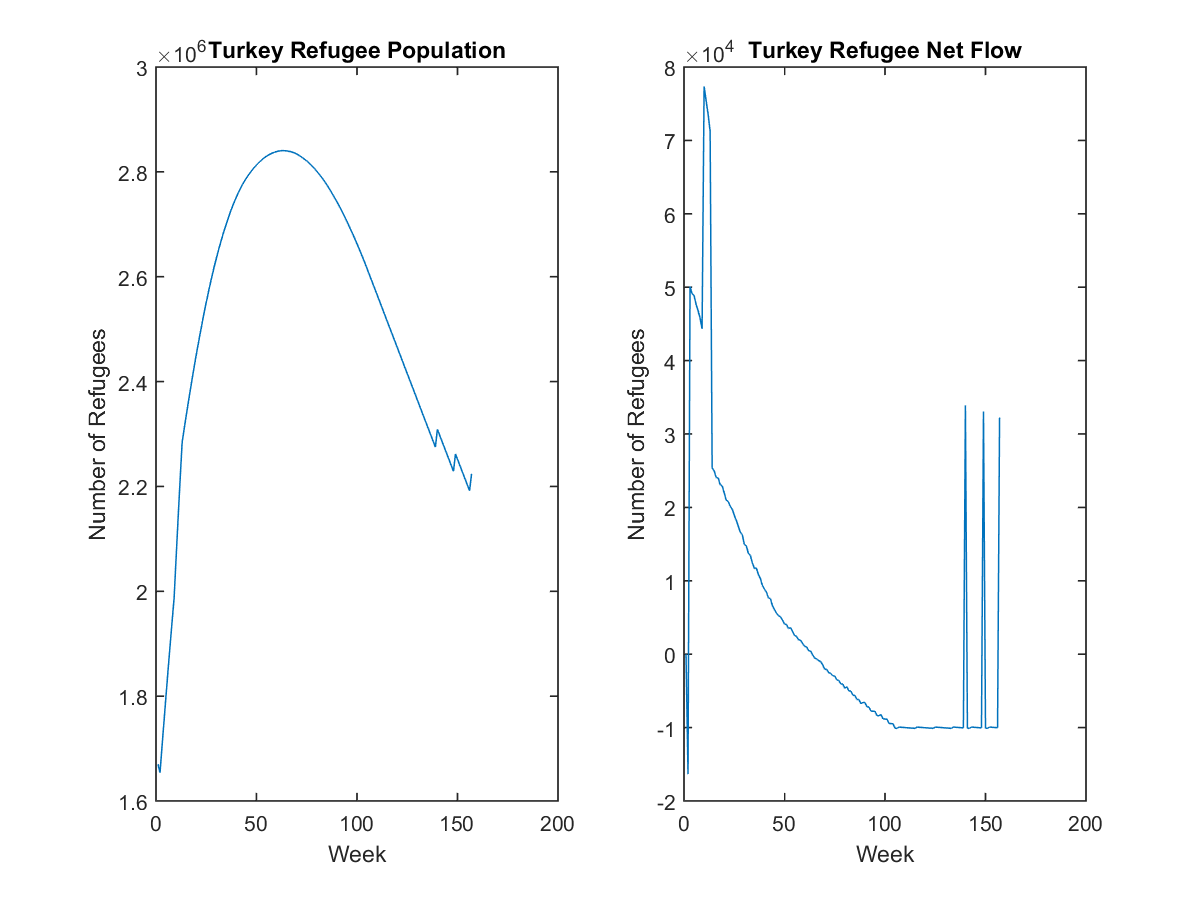
\includegraphics[width=.7\textwidth]{PostRefugeePlots/Turkey_RefugeePopandFlow.png}
    \caption [width=0.9\textwidth]{\centering Turkey refugee population and flow.}
\end{figure}

The flow of refugees to destination countries is delayed until later in the time frame. Sweden, for example, has a maximum inflow of refugees occurring within the second year of the model. This is likely due to the creation of the bottleneck in the hub countries, as well as the initial lack of resources to increase refugee capacity.

\begin{figure}[H]
    \centering
    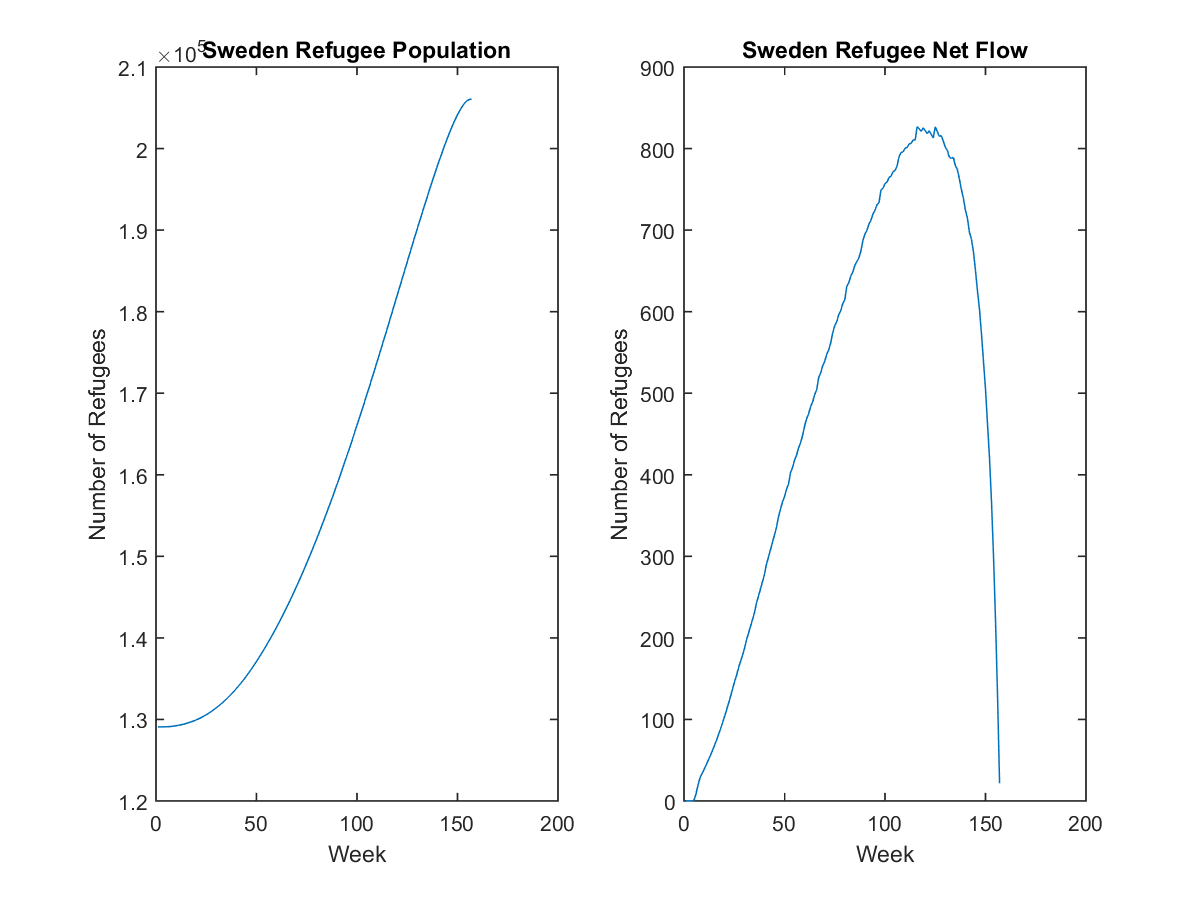
\includegraphics[width=.7\textwidth]{PostRefugeePlots/Sweden_RefugeePopandFlow.png}
    \caption [width=0.9\textwidth]{\centering Sweden refugee population and flow.}
\end{figure}

A look at the maximum inflow and outflow for each country shows that for optimal refugee movement, certain countries should be able to handle an inflow on the order of $10^5$. We see this occurring in major hub countries such as Turkey and Morocco. This is expected, as at the start of the crisis, and for many months following it, there is an almost endless queue of people wishing to flee.


\begin{figure}[H]
    \centering
    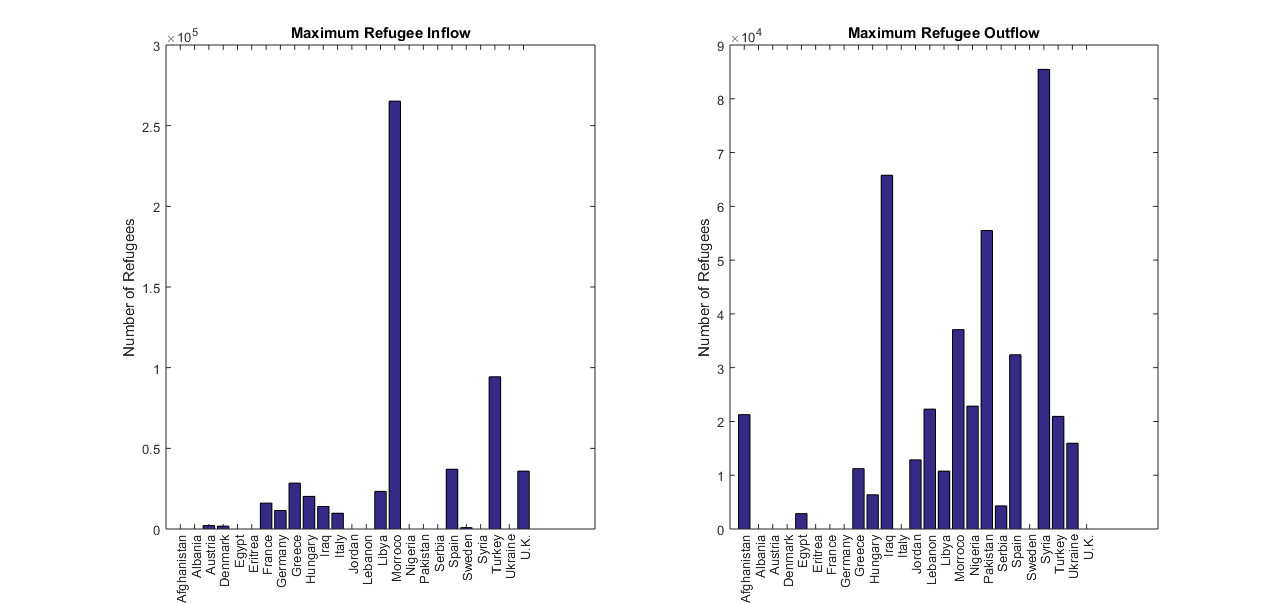
\includegraphics[width=\textwidth]{Sensitivity/baseflow.png}
    \caption [width=0.9\textwidth]{\centering Maximum inflow and outflow of refugees per location.}
\end{figure}

By the end of the time span, many of the refugees have been relocated to destination European countries. 

\begin{figure}[H]
    \centering
    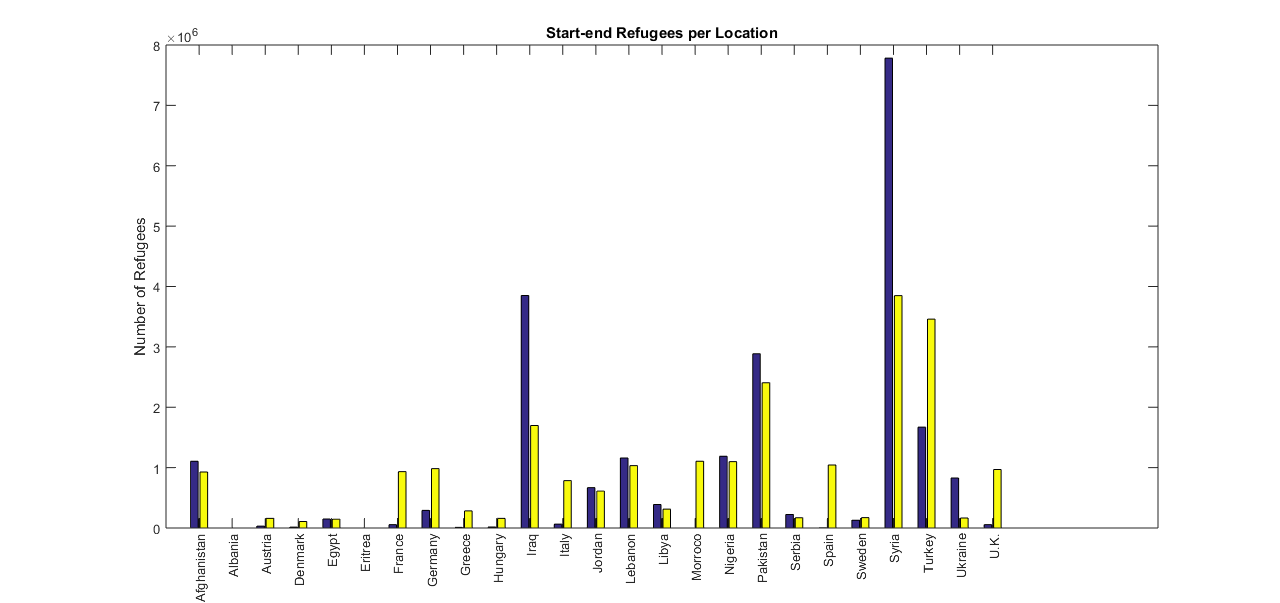
\includegraphics[width=\textwidth]{Sensitivity/basepop1.png}
    \caption [width=0.9\textwidth]{\centering The start (blue) and end (yellow) number of refugees per location.}
\end{figure}

The most optimal travel route for refugees is through Morocco and Spain with as many as 6.5 million refugees travelling this path.

\begin{figure}[H]
    \centering
    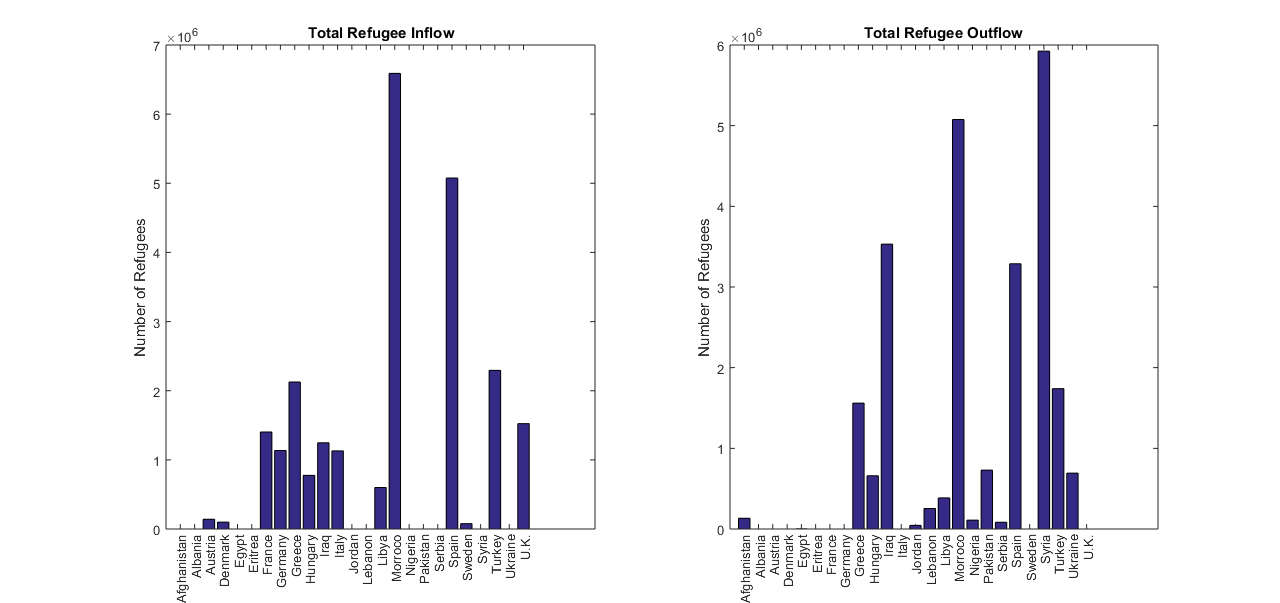
\includegraphics[width=\textwidth]{Sensitivity2/base.png}
    \caption [width=0.9\textwidth]{\centering Total inflow and outflow of each country.}
\end{figure}

\subsection{Sensitivity Analysis}

To test the effect of our assumptions on the model as a whole, we performed a sensitivity analysis on what we felt were three major components of the model that had to be assumed. These were: capacity for refugees, percentage of GDP used for internal aid, and a heavier penalty for traveling long distances.

\subsubsection{Sensitivity with respect to GDP}


\begin{figure}[H]
    \centering
    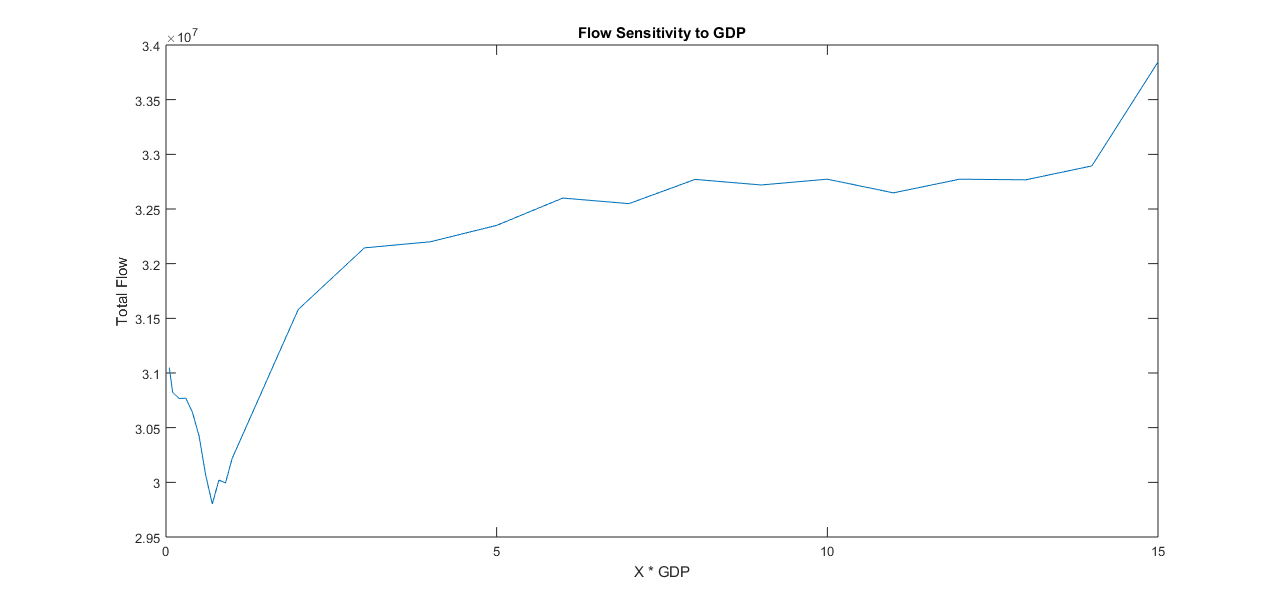
\includegraphics[width=0.7\textwidth]{Sensitivity3/sgdp.png}
    \caption [width=0.5\textwidth]{\centering Model flow sensitivity to GDP.}
\end{figure}

From the figure above, we can see that the flow is somewhat sensitive to the proportion of GDP that is spent on refugees within a country's borders. In fact, if the spending is very low, increasing it even by a small amount can have drastic effects, increasing flow by a great deal. However, this effect does not continue, and there seems to be a plateau hit before increasing substantially again. This is likely due to a maximum number of refugees moving to the country, and an equilibrium being reached between aid monies and GDP. However, after a certain point, internal spending once again drastically increases the draw of countries to refugees.

\subsubsection{Sensitivity with respect to Capacity for Refugees}

The flow of refugees remains fairly constant until a factor smaller than .3 of capacity is reached. This is expected, as the current total refugee population doesn't exceed the total capacity of our network and also reveals that the network can handle a larger refugee population. This mechanic could be used to implement exogenous events into our model. 

\begin{figure}[H]
    \centering
    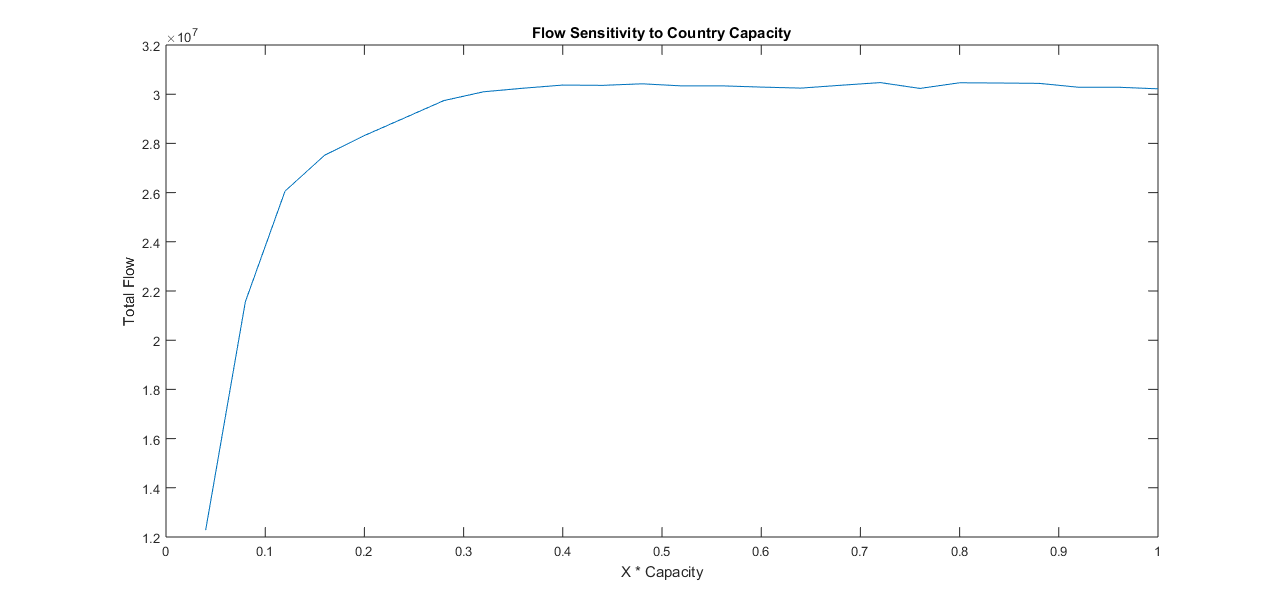
\includegraphics[width=0.7\textwidth]{Sensitivity3/scap.png}
    \caption [width=0.5\textwidth]{\centering Model flow sensitivity to country capacity.}
\end{figure}

\subsubsection{Sensitivity with respect to Distance}

Surprisingly, our model is completely insensitive to route distance. An explanation may be that the other costs of moving far outweigh the cost associated with distance. This also suggests that no matter the cost, refugees will find a way to flee from their home country in times of great crisis.

\begin{figure}[H]
    \centering
    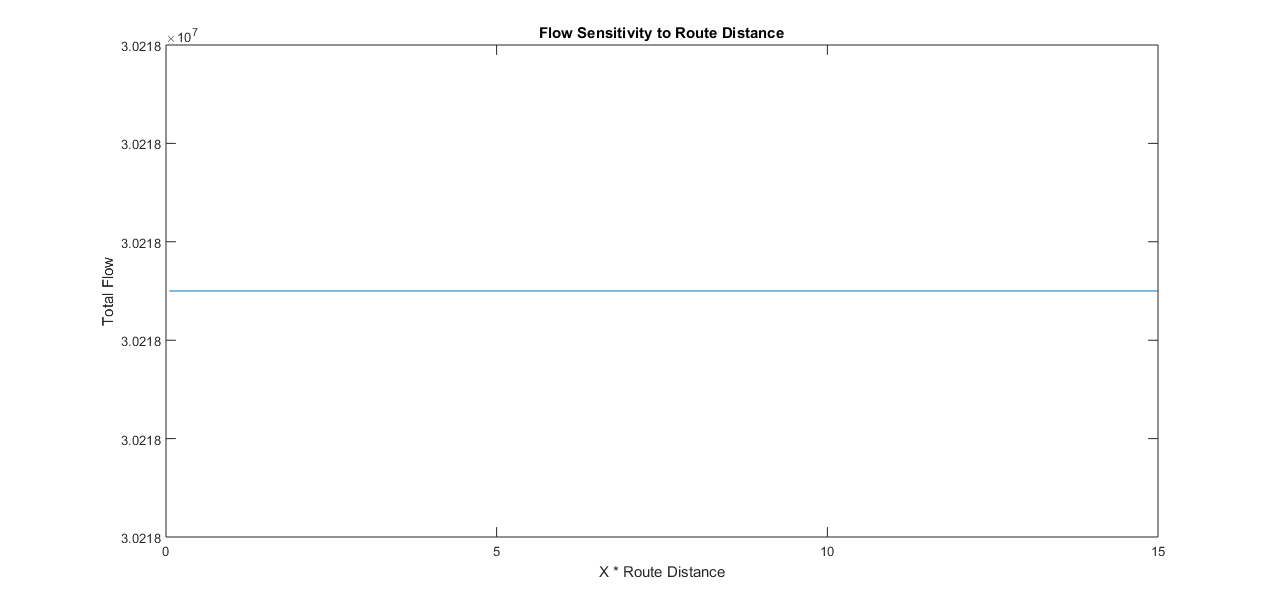
\includegraphics[width=0.7\textwidth]{Sensitivity3/sdist.png}
    \caption [width=0.5\textwidth]{\centering Model flow sensitivity to route distance.}
\end{figure}




\subsection{Scalability}
Our model is able to handle larger refugee populations tested to a scale of 15 times the 2014 values. Below we can see that increasing the number of initial refugees by varying factors increases the overall flow in the model. However, it seems to taper off as a threshold population is reached, where the network becomes saturated with refugees and refugees have no good choices for their movement, or they become stuck oscillating between locations.

\begin{figure}[H]
    \centering
    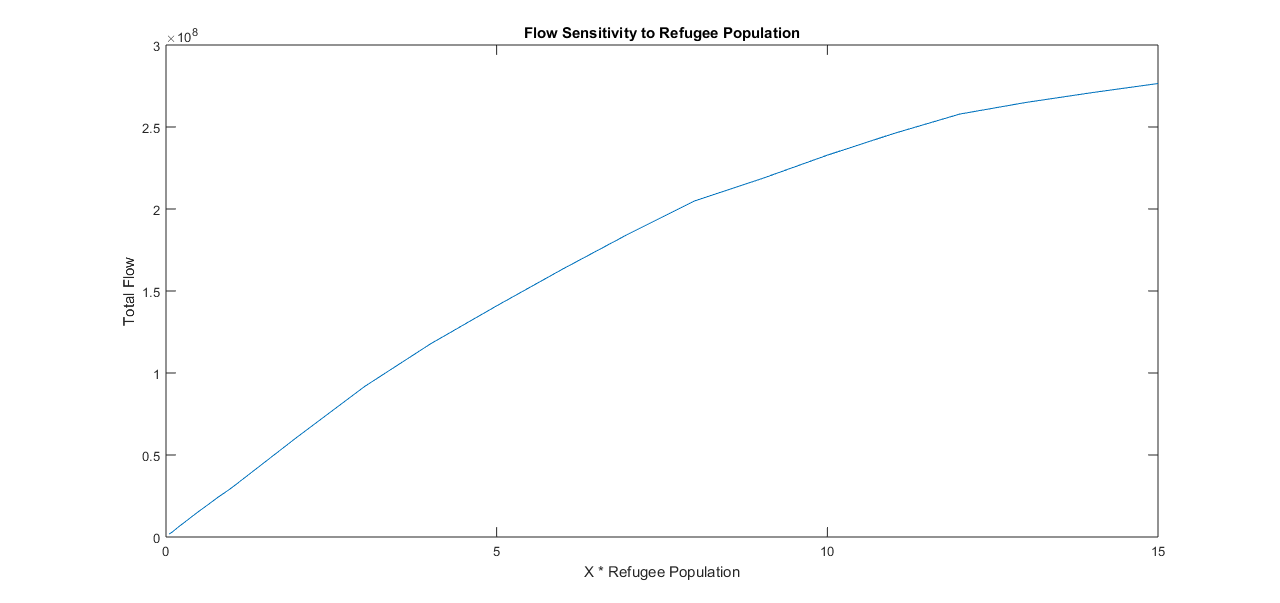
\includegraphics[width=\textwidth]{Sensitivity3/srpop.png}
    \caption [width=0.6\textwidth]{\centering Model flow sensitivity to population.}
\end{figure}



\subsection{Strengths}
\begin{itemize}
    \item This model incorporates a wide range of factors to simulate a realistic decision making process of refugees. For example, indexes such as HDI and FSI are used to determine the "utility" of the country in question.
    \item The calculated flows of refugees match real world data and simulate well the movement of refugees between countries.
    \item This model incorporates easily accessible data, which is available for all countries. Thus the model can easily be adapted to incorporate recent trends or to add more countries to the network.
    \item In each time step, our model moves people first, and then resources, creating the effect of resources "chasing" refugees. This creates a realistic simulation of the allocation of resources to help those who most need them, since a crisis would start unexpectedly and then resources would be focused on stabilizing the situation.
    \item The realistic sensitivity of refugee flow to country capacity could easily be used as a mechanic for implement exogenous events into the model.
\end{itemize}


\subsection{Weaknesses}
\begin{itemize}
    \item Certain of the population graphs have odd patterns, which suggests that some coefficients need to be calibrated further.
    \item Our model liquefies all resources (i.e., considers all resources in terms of monetary value). This may not be as accurate as considering each type of resource separately.
    \item The model has to perform its calculations in a discrete step instead of continuous, so there are waves of refugees each step, and thus some of the intricacies of travel such as smaller waves are washed out from the model.
    \item Distance doesn't affect model outcome. 
\end{itemize}

\section{Informed Policy}
To develop policy, we must first look at where the model says would be the best locations to allocate resources to. From the figures below, we can see that not all nodes immediately need aid, and in fact, some locations where one would expect to send aid are not the places that require aid. Spain, for instance is not a country that one would expect to require funds, however, when one realizes that it must brace itself for the enormous influx of refugees that are spilling over Europe's borders, it begins to make sense. One country that we would expect to require funds would be debt-saddled Greece. However, the model shows that Greece is truly a transient location in that refugees come and leave almost immediately, there are hardly any standing populations of refugees, thus there is not a vast requirement for funds to sustain them. However, countries where they are less likely to move from once they arrive will require significant funding, as well as European countries that will accepted increased numbers of refugees, such as France or Italy.

\begin{figure}[H]
    \centering
    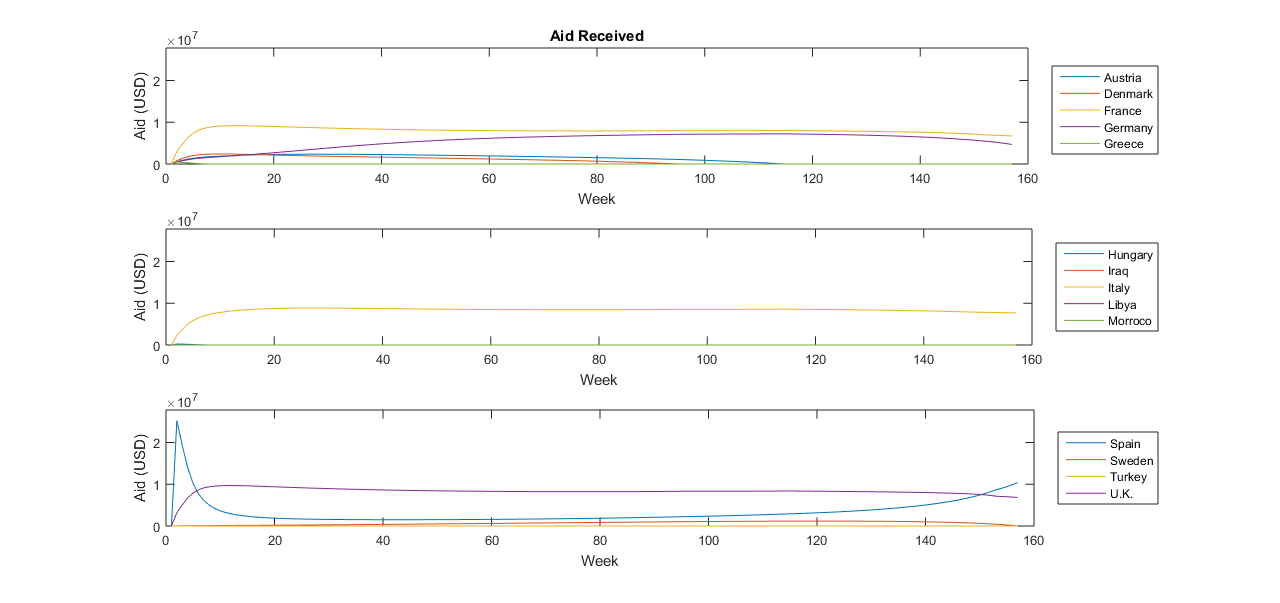
\includegraphics[width=\textwidth]{aid/aidcountrytime.png}
    \caption [width=0.9\textwidth]{\centering The evolution of aid distribution over time}
\end{figure}

\begin{figure}[H]
    \centering
    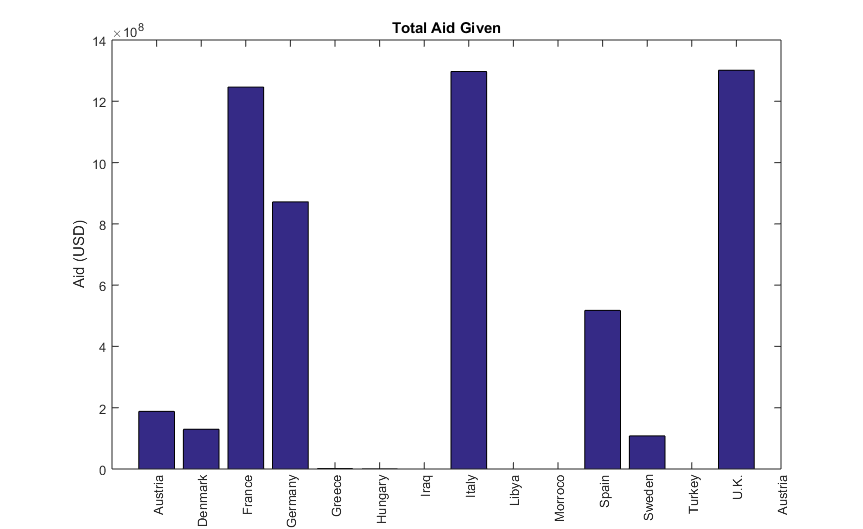
\includegraphics[width=.7\textwidth]{aid/totalaidgiven.png}
    \caption [width=0.9\textwidth]{\centering Comparison of total aid received for recipient countries}
\end{figure}

From this data, we can generate policies to handle a crisis such as this: 
\begin{itemize}
    \item Prioritize countries that harbor standing populations of refugees rather countries that handle the most refugees.
    \item Supplement domestic spending on refugees with international aid to encourage raised capacities for refugees in developed countries to allow for resettlement of increased numbers of refugees.
    \item Do not give all aid away at one time, rather allow the distribution of aid to evolve with the dynamics of the crisis for maximum efficiency.
    \item Anticipate arrival of refugees regardless of conditions of travel. If funds are produced in excess once the crisis begins, then begin to fund better infrastructure, but do not waste precious funds with this in the early stages of a crisis.
    
    This last policy suggestion comes with some stipulations. In the middle of a crisis, it would be incredibly inefficient to spend aid money on developing travel routes, as people will find their way, regardless of conditions. Aid money should be focused on settling refugees, which will increase the overall stability of a region. \\
    However, if the amount of refugees flocking to a region becomes such that it threatens to destabilize the entire region, it might be necessary to expand travel routes. Consider if the scale of the refugee crisis were 10 times what it were now. In this case, it would be worth the immense cost to build new transportation routes or develop new routes to countries like China or the United States.
    
    Note: The total amount of funds allocated to each country over three years can be found in Figure 4 of the appendix.
\end{itemize}


\section{Exogenous Events}
The recent influx in refugees is symptomatic of political unrest throughout the world. Thus, it is likely that a surge of refugees would be accompanied by other major disruptions, such as terrorist attacks. Our model accounts for these disruptions, just as there would be real life consequences of such events such as shifts in policy, shifts in attitudes, and likely closure of borders. \\
If a major disruption occurred, it is likely that the first model parameter to change would be the allocation of international aid money. These resources would likely be partially reallocated to help the affected area, and thus the amount available to help refugees would decrease. \\
In addition, it is likely that, over time, the FSI and HDI in the area of any major disruption would be affected. Disruptions such as terrorists attacks decrease the security and stability of a country and effect the standard of living there. Also, affected countries may adopt more strict screening of those they allow in, which would likely drop the refugee cap.  \\
All of these changes in parameters would affect the movement of refugees throughout the model. As the area of disruption experienced a decrease in standard living and a possible lowering of refugee cap, refugees would be discouraged from travelling to that country, and any refugees inside that country might be encouraged to travel away. This would increase the number of refugees in the countries surrounding the center of the disruption. However, as refugees left the area, the lowered standard of living would pull resources toward the center of disruption. As the resources help the affected people, the standard of living should increase, which would eventually begin to pull refugees back. \\
However, the policies we recommend should be fairly resilient to such a event. Through our policies, we encourage refugees to settle in the most stable countries possible. Stable countries are much less likely to experience a major disruption. Thus, a major disruption would not displace an overwhelming amount of people, and those who are displaced could be absorbed into the nearest countries.

\section{Conclusions}
The surge of refugees throughout Europe is a serious concern that must be addressed through effective policy and resource allocation. \\
To this aim, we have developed a robust model that simulates the movement of refugees and then allocates resources in the most efficient way possible to stabilize the situation as quickly as possible. From this model, we were able to determine that there is a bottleneck forming around hub countries such as Hungary, Morocco, Greece, and Turkey who handle a lot of refugees in their roles as halfway homes between North Africa or the Middle East and Europe. Additionally, the model showed that aid should be distributed to countries that will accumulate large standing populations of refugees, such as Spain. We found that refugees will find a way to move through the network to their desired country one way or another, the potential risk death is far outweighed by the potential gain of arriving in a better country. A result of this is that aid should be directed towards European countries to coax them into opening their borders to allow more refugees to stay in their country. If the refugees are capable of finding a way to Europe on their own, resources should be spent making sure that they are not turned away or left standing in countries such as Turkey, as this is not ideal for either party and could potentially destabilize the region further. In conclusion, we developed a model that simulates refugee movements based on their decision making processes, and furthermore provides a guideline for how aid should be distributed to stabilize the situation most efficiently and effectively.


\section{Further Work}
Though our model is a robust simulation for the movement of refugees and the responsive movement of resources, there are areas for further work:
\begin{enumerate}
    \item Determine threshold population of refugees for countries in crisis, i.e. the number of refugees they can produce before the entire surrounding region folds upon itself.
    \item In our model, our time step emulates a week in the real world. However, further work could be done to calibrate the time step for the model by adjusting flow rates on paths, possibly with a max flow on each route (in other words, imposing a  limit on the amount of people that can move each given time step).
    \item In our model, we combined all the resources a refugee might need (food, water, medicine, housing) and represented them through a monetary value. However, it would be interesting to consider each resource on its own.
    \item Additionally, work could be done on producing a continuous model of refugee movement, so that instead of waves every time step, there are multiple convoys dispatched every time step.
    \item The individual factors that make up HDI and FSI could be updated at each time step to predict evolution of countries throughout the crisis.
\end{enumerate}


\pagebreak

\newpage
\appendix 
\section*{Appendix}
\setcounter{figure}{0}  

\centering
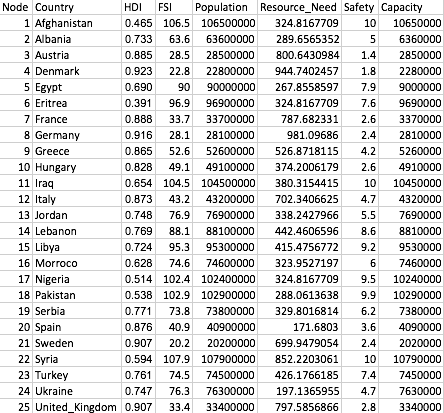
\includegraphics[width=3in, height=3in]{data_value2.png}
\captionof{figure}{\centering Table of values used to calculate coefficients for each node.}


\begin{equation*}
    \left(\begin{array}{ccccccccccccccccccccccccc} 1 & 0 & 0 & 0 & 0 & 0 & 0 & 0 & 0 & 0 & 0 & 0 & 0 & 0 & 1 & 1 & 0 & 0 & 0 & 0 & 0 & 0 & 1 & 0 & 0\\ 0 & 1 & 0 & 0 & 0 & 0 & 0 & 0 & 1 & 0 & 0 & 0 & 0 & 0 & 0 & 0 & 0 & 0 & 0 & 0 & 0 & 0 & 0 & 0 & 0\\ 0 & 0 & 1 & 0 & 0 & 0 & 0 & 0 & 0 & 0 & 0 & 0 & 0 & 0 & 0 & 0 & 0 & 0 & 0 & 0 & 0 & 0 & 0 & 0 & 0\\ 0 & 0 & 0 & 1 & 0 & 0 & 0 & 0 & 0 & 0 & 0 & 0 & 0 & 0 & 0 & 0 & 0 & 0 & 0 & 0 & 0 & 0 & 0 & 0 & 0\\ 0 & 0 & 0 & 0 & 1 & 0 & 0 & 0 & 0 & 0 & 0 & 0 & 0 & 0 & 1 & 1 & 0 & 0 & 0 & 0 & 0 & 0 & 1 & 0 & 0\\ 0 & 0 & 0 & 0 & 0 & 1 & 0 & 0 & 0 & 0 & 0 & 0 & 0 & 0 & 1 & 1 & 0 & 0 & 0 & 0 & 0 & 0 & 0 & 0 & 0\\ 0 & 0 & 0 & 0 & 0 & 0 & 1 & 0 & 0 & 0 & 0 & 0 & 0 & 0 & 0 & 0 & 0 & 0 & 0 & 0 & 0 & 0 & 0 & 0 & 0\\ 0 & 0 & 0 & 0 & 0 & 0 & 0 & 1 & 0 & 0 & 0 & 0 & 0 & 0 & 0 & 0 & 0 & 0 & 0 & 0 & 0 & 0 & 0 & 0 & 0\\ 0 & 0 & 1 & 1 & 0 & 0 & 1 & 1 & 1 & 0 & 0 & 1 & 0 & 0 & 0 & 0 & 0 & 0 & 0 & 0 & 1 & 0 & 0 & 0 & 1\\ 0 & 0 & 1 & 1 & 0 & 0 & 1 & 1 & 0 & 1 & 0 & 1 & 0 & 0 & 0 & 0 & 0 & 0 & 0 & 0 & 1 & 0 & 0 & 0 & 1\\ 0 & 0 & 0 & 0 & 0 & 0 & 0 & 0 & 0 & 0 & 1 & 0 & 0 & 0 & 1 & 1 & 0 & 0 & 0 & 0 & 0 & 0 & 1 & 0 & 0\\ 0 & 0 & 0 & 0 & 0 & 0 & 0 & 0 & 0 & 0 & 0 & 1 & 0 & 0 & 0 & 0 & 0 & 0 & 0 & 0 & 0 & 0 & 0 & 0 & 0\\ 0 & 0 & 0 & 0 & 0 & 0 & 0 & 0 & 0 & 0 & 0 & 0 & 1 & 0 & 1 & 1 & 0 & 0 & 0 & 0 & 0 & 0 & 1 & 0 & 0\\ 0 & 0 & 0 & 0 & 0 & 0 & 0 & 0 & 0 & 0 & 0 & 0 & 0 & 1 & 1 & 1 & 0 & 0 & 0 & 0 & 0 & 0 & 1 & 0 & 0\\ 0 & 0 & 0 & 0 & 0 & 0 & 0 & 0 & 1 & 0 & 0 & 0 & 0 & 0 & 1 & 0 & 0 & 0 & 0 & 0 & 0 & 0 & 0 & 0 & 0\\ 0 & 0 & 0 & 0 & 0 & 0 & 0 & 0 & 0 & 0 & 0 & 0 & 0 & 0 & 0 & 1 & 0 & 0 & 0 & 1 & 0 & 0 & 0 & 0 & 0\\ 0 & 0 & 0 & 0 & 0 & 0 & 0 & 0 & 0 & 0 & 0 & 0 & 0 & 0 & 1 & 1 & 1 & 0 & 0 & 0 & 0 & 0 & 0 & 0 & 0\\ 0 & 0 & 0 & 0 & 0 & 0 & 0 & 0 & 0 & 0 & 0 & 0 & 0 & 0 & 1 & 1 & 0 & 1 & 0 & 0 & 0 & 0 & 1 & 0 & 0\\ 0 & 0 & 0 & 0 & 0 & 0 & 0 & 0 & 0 & 1 & 0 & 0 & 0 & 0 & 0 & 0 & 0 & 0 & 1 & 0 & 0 & 0 & 0 & 0 & 0\\ 0 & 0 & 1 & 1 & 0 & 0 & 1 & 1 & 0 & 0 & 0 & 1 & 0 & 0 & 0 & 0 & 0 & 0 & 0 & 1 & 1 & 0 & 0 & 0 & 1\\ 0 & 0 & 0 & 0 & 0 & 0 & 0 & 0 & 0 & 0 & 0 & 0 & 0 & 0 & 0 & 0 & 0 & 0 & 0 & 0 & 1 & 0 & 0 & 0 & 0\\ 0 & 0 & 0 & 0 & 0 & 0 & 0 & 0 & 0 & 0 & 1 & 0 & 0 & 0 & 1 & 1 & 0 & 0 & 0 & 0 & 0 & 1 & 1 & 0 & 0\\ 0 & 0 & 0 & 0 & 0 & 0 & 0 & 0 & 1 & 0 & 0 & 0 & 0 & 0 & 0 & 0 & 0 & 0 & 0 & 0 & 0 & 0 & 1 & 0 & 0\\ 0 & 0 & 0 & 0 & 0 & 0 & 0 & 0 & 0 & 1 & 0 & 0 & 0 & 0 & 0 & 0 & 0 & 0 & 0 & 0 & 0 & 0 & 0 & 1 & 0\\ 0 & 0 & 0 & 0 & 0 & 0 & 0 & 0 & 0 & 0 & 0 & 0 & 0 & 0 & 0 & 0 & 0 & 0 & 0 & 0 & 0 & 0 & 0 & 0 & 1 \end{array}\right)
\end{equation*}
\captionof{figure}{Adjacency Matrix for the Refugee Movement Network}


\begin{equation*}
    \left(\begin{array}{cccccccccccccccccccccccccc} 0 & 0 & 0 & 0 & 0 & 0 & 0 & 0 & 0 & 0 & 0 & 0 & 0 & 0 & 0 & 0 & 0 & 0 & 0 & 0 & 0 & 0 & 0 & 0 & 0 & 0\\ 0 & 0 & 0 & 0 & 0 & 0 & 0 & 0 & 0 & 0 & 0 & 0 & 0 & 0 & 0 & 0 & 0 & 0 & 0 & 0 & 0 & 0 & 0 & 0 & 0 & 0\\ 0 & 0 & 0 & 0 & 0 & 0 & 0 & 0 & 0 & 0 & 0 & 0 & 0 & 0 & 0 & 0 & 0 & 0 & 0 & 0 & 0 & 0 & 0 & 0 & 0 & 0\\ 0 & 0 & 0 & 0 & 0 & 0 & 0 & 0 & 0 & 0 & 0 & 0 & 0 & 0 & 0 & 0 & 0 & 0 & 0 & 0 & 0 & 0 & 0 & 0 & 0 & 0\\ 0 & 0 & 0 & 0 & 0 & 0 & 0 & 0 & 0 & 0 & 0 & 0 & 0 & 0 & 0 & 0 & 0 & 0 & 0 & 0 & 0 & 0 & 0 & 0 & 0 & 0\\ 0 & 0 & 0 & 0 & 0 & 0 & 0 & 0 & 0 & 0 & 0 & 0 & 0 & 0 & 0 & 0 & 0 & 0 & 0 & 0 & 0 & 0 & 0 & 0 & 0 & 0\\ 0 & 0 & 0 & 0 & 0 & 0 & 0 & 0 & 0 & 0 & 0 & 0 & 0 & 0 & 0 & 0 & 0 & 0 & 0 & 0 & 0 & 0 & 0 & 0 & 0 & 0\\ 0 & 0 & 0 & 0 & 0 & 0 & 0 & 0 & 0 & 0 & 0 & 0 & 0 & 0 & 0 & 0 & 0 & 0 & 0 & 0 & 0 & 0 & 0 & 0 & 0 & 0\\ 0 & 0 & 0 & 0 & 0 & 0 & 0 & 0 & 0 & 0 & 0 & 0 & 0 & 0 & 0 & 0 & 0 & 0 & 0 & 0 & 0 & 0 & 0 & 0 & 0 & 0\\ 0 & 0 & 0 & 0 & 0 & 0 & 0 & 0 & 0 & 0 & 0 & 0 & 0 & 0 & 0 & 0 & 0 & 0 & 0 & 0 & 0 & 0 & 0 & 0 & 0 & 0\\ 0 & 0 & 0 & 0 & 0 & 0 & 0 & 0 & 0 & 0 & 0 & 0 & 0 & 0 & 0 & 0 & 0 & 0 & 0 & 0 & 0 & 0 & 0 & 0 & 0 & 0\\ 0 & 0 & 0 & 0 & 0 & 0 & 0 & 0 & 0 & 0 & 0 & 0 & 0 & 0 & 0 & 0 & 0 & 0 & 0 & 0 & 0 & 0 & 0 & 0 & 0 & 0\\ 0 & 0 & 0 & 0 & 0 & 0 & 0 & 0 & 0 & 0 & 0 & 0 & 0 & 0 & 0 & 0 & 0 & 0 & 0 & 0 & 0 & 0 & 0 & 0 & 0 & 0\\ 0 & 0 & 0 & 0 & 0 & 0 & 0 & 0 & 0 & 0 & 0 & 0 & 0 & 0 & 0 & 0 & 0 & 0 & 0 & 0 & 0 & 0 & 0 & 0 & 0 & 0\\ 0 & 0 & 0 & 0 & 0 & 0 & 0 & 0 & 0 & 0 & 0 & 0 & 0 & 0 & 0 & 0 & 0 & 0 & 0 & 0 & 0 & 0 & 0 & 0 & 0 & 0\\ 0 & 0 & 0 & 0 & 0 & 0 & 0 & 0 & 0 & 0 & 0 & 0 & 0 & 0 & 0 & 0 & 0 & 0 & 0 & 0 & 0 & 0 & 0 & 0 & 0 & 0\\ 0 & 0 & 0 & 0 & 0 & 0 & 0 & 0 & 0 & 0 & 0 & 0 & 0 & 0 & 0 & 0 & 0 & 0 & 0 & 0 & 0 & 0 & 0 & 0 & 0 & 0\\ 0 & 0 & 0 & 0 & 0 & 0 & 0 & 0 & 0 & 0 & 0 & 0 & 0 & 0 & 0 & 0 & 0 & 0 & 0 & 0 & 0 & 0 & 0 & 0 & 0 & 0\\ 0 & 0 & 0 & 0 & 0 & 0 & 0 & 0 & 0 & 0 & 0 & 0 & 0 & 0 & 0 & 0 & 0 & 0 & 0 & 0 & 0 & 0 & 0 & 0 & 0 & 0\\ 0 & 0 & 0 & 0 & 0 & 0 & 0 & 0 & 0 & 0 & 0 & 0 & 0 & 0 & 0 & 0 & 0 & 0 & 0 & 0 & 0 & 0 & 0 & 0 & 0 & 0\\ 0 & 0 & 0 & 0 & 0 & 0 & 0 & 0 & 0 & 0 & 0 & 0 & 0 & 0 & 0 & 0 & 0 & 0 & 0 & 0 & 0 & 0 & 0 & 0 & 0 & 0\\ 0 & 0 & 0 & 0 & 0 & 0 & 0 & 0 & 0 & 0 & 0 & 0 & 0 & 0 & 0 & 0 & 0 & 0 & 0 & 0 & 0 & 0 & 0 & 0 & 0 & 0\\ 0 & 0 & 0 & 0 & 0 & 0 & 0 & 0 & 0 & 0 & 0 & 0 & 0 & 0 & 0 & 0 & 0 & 0 & 0 & 0 & 0 & 0 & 0 & 0 & 0 & 0\\ 0 & 0 & 0 & 0 & 0 & 0 & 0 & 0 & 0 & 0 & 0 & 0 & 0 & 0 & 0 & 0 & 0 & 0 & 0 & 0 & 0 & 0 & 0 & 0 & 0 & 0\\ 0 & 0 & 0 & 0 & 0 & 0 & 0 & 0 & 0 & 0 & 0 & 0 & 0 & 0 & 0 & 0 & 0 & 0 & 0 & 0 & 0 & 0 & 0 & 0 & 0 & 0\\ 0 & 0 & 1 & 1 & 0 & 0 & 1 & 1 & 1 & 1 & 1 & 1 & 0 & 0 & 1 & 1 & 0 & 0 & 0 & 1 & 1 & 0 & 1 & 0 & 1 & 0 \end{array}\right)
\captionof{figure}{Adjacency Matrix for the Resource Distribution Network}

\newpage
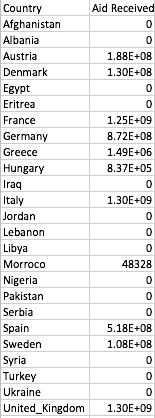
\includegraphics[width=1in, height=2.5in]{aidover3.png}
\captionof{figure}{\centering Table of amounts (usd) of foreign aid each country recieves over 3 years}

\end{equation*}

\pagebreak

\newpage
%\bibsection
\nocite{*}
\bibliography{mybibliography}
\bibliographystyle{plain}

\end{document}